% Introduction
\chapter{Introduction}

\nek{} \cite{CantwellMCBRMGYLEJXMENVBKS2015}, is an open-source software framework designed to support the development of 
high-performance scalable solvers for partial differential equations using the spectral/{\em hp\/} element method.   
What in part makes \nek{} unique is that it is  
an initiative to overcome the mathematical complexities of the methods by encapsulating them within an efficient cross-platform {\em C++} software environment, consequently making the techniques more accessible to the broader scientific and industrial communities. The software supports a variety of discretization techniques and 
implementation strategies \cite{VosSK2010,CantwellSKK2011a,CantwellSKK2011b,BolisCKS2014},
supporting methods research as well as application-focused computation, and the multi-layered structure of the framework allows the user to embrace as much or as little of the complexity as they need. The libraries capture the mathematical constructs of spectral/{\em hp\/} element methods in the form of a hierarchy of {\em C++} components, while the associated collection of pre-written PDE solvers provides out-of-the-box functionality across a range of application areas, as well as a template for users who wish to develop solutions for addressing questions in their own scientific domains.

% Overview of Nektar++ and its goals/features
The cross-platform nature of the software libraries enables the rapid development of solvers for use in a wide variety of computing environments. The code accommodates both small research problems, suitable for desktop computers, and large-scale industrial simulations, requiring modern HPC infrastructure, where there is a need to maintain efficiency and scalability up to many thousands of processor cores.

\nek{} provides a single codebase with the following key features:
\begin{itemize}
  \item Arbitrary-order \shp{} element discretisations in one, two and three
  dimensions;
  \item Support for variable polynomial order in space and heterogeneous
  polynomial order within two- and three-dimensional elements;
  \item High-order representation of the geometry;
  \item Continuous Galerkin, discontinuous Galerkin and hybridised discontinuous
  Galerkin projections;
  \item Support for a Fourier extension of the spectral element mesh;
  \item Support for a range of linear solvers and preconditioners;
  \item Multiple implementation strategies for achieving linear algebra
  performance on a range of platforms;
  \item Efficient parallel communication using MPI showing strong scaling up to
  8192-cores on Archer, the UK national HPC system;
  \item A range of time integration schemes implemented using generalised linear
  methods; and
  \item Cross-platform support for Linux, OS X and Windows operating
  systems.
\end{itemize}

In addition to the core functionality listed above, \nek{} includes a
number of solvers covering a range of application areas. A range
of pre-processing and post-processing utilities are also included with support
for popular mesh and visualization formats, and an extensive test suite ensures
the robustness of the core functionality.


%%%%%%%%%%%%%%%%%%%%%%%%%%%%%%%%%%%%%%%%%%%%%%%%%%

\section{The {\em Ethos} of Nektar++}


As with any research effort, one is required to decide on a set of guiding principles that will 
drive the investigation.  Similarly with a software development effort of this form, we  
spent considerable time early on considering which aspects we wanted to be distinctive about {\nek} and also
what guiding principles would be most suitable to support both the goals and the boundaries of what
we wanted to do.  We did this for at least two reasons:  (1) We acknowledged then and now that
there are various software packages and open-source efforts that deal with finite element frameworks,
and so we wanted to be able to understand and express to people those things we thought were
distinctive to us -- that is, our ``selling points''.  (2) We also acknowledged, from our own experience
on software projects, that if we did not set up some collection of guiding principles for our work, that
we would gravitate towards trying to be ``all things to all men", and in doing so be at odds with the
first item.  Below are a list of the guiding principles, the ``ethos'', of the Nektar++ software development
effort.

\paragraph{Principles:}
The following are our three guiding principles for {\nek} which respect (1) above:

\begin{itemize}
\item \textbf{Efficiently:} {\nek} was to be a ``true'' high-order code.  ``True'' is put in quotations because we acknowledge
that high-order means different things to different communities.  Based upon a review of the literature, we 
came to the conclusion that part of our {\em h-to-p} philosophy should be that we accommodate polynomial
degrees ranging from zero (finite volumes) or one (traditional linear finite elements) up to what is considered
``spectral'' (pseudospectral) orders of 16$^{th}$ degree.  As part of our early work \cite{VosSK2010}, we established that in
order to span this range of polynomial degrees and attempt to maintain some level of computational 
efficiency, we would need to develop {\em order-aware} algorithms:  that is, we would need to utilize
different (equivalent) algorithms appropriate for a particular order.  This principle was the starting point
of our {\em h-to-p efficiently} branding and continues to be a driving principle of our work. 

\item \textbf{Transparently:} {\nek} was to be agnostic as to what the ``right'' way to discretize a partial differential equation (PDE).
``Right'' is put in quotations to acknowledge that like the issue of polynomial order, there appear to be different
``camps'' who hold very strong views as to which discretization method should be used.   Some might concede that
continuous Galerkin methods are very natural for elliptic and parabolic PDEs and then work very laboriously to 
shoehorn all mixed-type PDEs (such as the incompressible Navier-Stokes equations) into this form.  This holds
true (similarly) for finite volume and dG proponents with regards to hyperbolic problems (and those systems that are
dominated by hyperbolicity).  Our goal was to be a high-order finite element framework that allowed users to experiment with
continuous Galerkin (cG) and discontinuous Galerkin (dG) methods.  After our original developments, we incorporated 
Flux-Reconstruction Methods (FR Methods) into our framework; this confirmed that generality of our approach as our
underlying library components merely needed new features added to accommodate the FR perspective on dG methods.
As stated earlier, this is in part why we use the term \shp{} as it allows us to capture all these various methods (e.g., cG, dG and FR)
under one common element-and-order terminology.

\item \textbf{Seamlessly:}  {\nek} was to be a code that could run from the desktop (or laptop) to exascale, seamlessly.  It was our
observation that many {\em grand challenge} efforts target petascale and exascale computing, with the idea that in the future
what is done now on a supercomputer will be done on the desktop.  The supercomputer of today is in a rack within five
years and on our desktop in ten years.  However, we also acknowledged that many of our end users were interested in computing
{\em now}.  That is, following from their engineering tradition they had an engineering or science problem to solve, and they wanted 
the ability to run on machines ranging from their laptops to exascale as the problem demanded.  Not all problems fit on your laptop, 
and yet not all problems are exascale problems.  Like with our {\em h-to-p efficiently} approach, we wanted our algorithms and code
development to allow a range of choices in the hands of the engineer.
\end{itemize}

Based upon these principles, our long-term vision is a software framework that allows the engineer the flexibility to make all
these critical choices (elemental discretization, polynomial order, discretization methodology, algorithms to employ, and 
architecture-specific details) while at the same time having {\em smart and adaptive defaults}.  That is, we want to 
accommodate both the engineer that wants control over all the various knobs that must be set to actualize a simulation run
and the engineer that wants to remain at the high-level and let the software system choose what is best in terms of discretization,
polynomial order, algorithm choice, etc.  We want the flexibility to self tune, while targeting auto-tuning.

The three items above denote the principles of our development efforts.  We now present the ``guardrails''.  By guardrails, we mean
the guidelines we use to help steer us along towards our goal as stated above.  These are not meant to be absolutes necessarily,
but are considerations we often use to try to keep us on track in terms of respecting our three guiding principles above.

\paragraph{Guardrails:}

\begin{itemize}
\item We are principally concerned with advection-reaction-diffusion and conservation law problems.   There are many
simulation codes that are deal with solid mechanics, and we did not see ourselves as being a competitor with them.  As such,
we did not initially construct our framework to inherently deal with $H-div$ and $H-curl$ spaces (and their respective element types).
Our perspective was to hold a system of scalar fields and, as needed, constrain them to respect certain mathematical properties.  

\item We rely heavily on the ability to do tensor-product-based quadrature.  Although our more recent additions to the Point and Basis
information within our library allows for unstructured quadrature, many of our algorithms are designed to try to capitalize on
tensor-product properties.

\item As we said earlier, we have designed our code to run at a range of orders, from one to sixteen.  However, we acknowledge that 
for many simulation regimes, we often do not run at the lowest and/or the highest orders.  For many applications, the sweet spot seems
to be polynomials of degree four through eight.  At the present time, a reasonable amount of time and effort has been spent optimizing
for this range.

\item The robustness of our testing is often dictated by the application areas that have funded our code development.  At the present
time, our incompressible Navier-Stokes solver is probably the most tested of our solvers, followed by our ADR solver.  We make
every attempt to test our codes thoroughly; however we benefit greatly from various users ``stress-testing'' our codes and providing 
feedback on things we can improve (or better yet, suggesting coding solutions).
\end{itemize}


%%%%%%%%%%%%%%%%%%%%%%%%%%%%%%%%%%%%%%%%%%%%%%%%%%

\section{The Structure of Nektar++}

When we speak of {\nek}, it often means different things to different people, all under an umbrella of code.  For the founders of {\nek}, 
the view was that the core of {\nek} was the library, and that everything else was to be built around or on top of our basic \shp{} framework.
For others, the heart of {\nek} are its solvers -- the collection of simulation codes, built upon the library, that enable users to solve
science and engineering problems.   For a smaller group of people, it is all the add-ons that we provide in our utilities, from our
mesh generation techniques to our visualization software ideas.   

For the purposes of this document, we will structure our discussions into three main parts:  library functionality, solvers and utilities.  In this
section, we will provide an overview of the structure of the libraries.  We will start by giving a quick overview of the basic subdirectories
contained within {\em library} and their purpose.  We will then provide a bottom-up description of how the library can be viewed, as well
as a top-down perspective.  Each perspective (bottom-up or top-down) is fully consistent with each other; the advantage of these approaches
is that they help the future developer understand the library as someone trying to build up towards our solvers, or conversely someone trying
to understand our solver functionality having already been a solver user and now trying to understand the library components on which it was built.

The basic subdirectories with the {\em library} are as follows:

\noindent{\textbf{LibUtilities:}}  This library contains all the basic mathematical and computer science building blocks of the {\nek} code.

\noindent{\textbf{StdRegions:}} This library contains the objects that express ``standard region'' data and operations.  In one dimension, this is the StdSegment.  In two 
dimensions, this is the StdTri (Triangle) and StdQuad (Quadrilateral).  In three dimensions, this is the StdTet (Tetrahedra), 
StdHex (Hexahedra), StdPrism (Prism) and StdPyr (Pyramid).  These represent the seven different standardized reference regions over which 
we support differentiation and integration. 

\noindent{\textbf{SpatialDomains:}} This library contains the mesh and elemental geometric information.  In particular, this part of the library deals with the basic mesh 
data structures, and the mapping information (such as Jacobians) from StdRegions to LocalRegions.

\noindent{\textbf{LocalRegions:}}  This library contains objects that express data and operations on individual physical elements of the computational mesh.  Local regions are \shp{} elements in
world-space (either straight-/planar-sided or curved-sided).  Using {\em C++} terminology, a local region object {\em is-a} standard region object and {\em has-a} spatial domain object.

\noindent{\textbf{MultiRegions:}} This library holds the data structures that represent sets of elements (local regions).  At the most fundamental 
level, these represent the union of local regions into a (geometrically-contiguous) space.  By specifying the interaction of these elements, the function space they represent and/or the approximation method is defined.  It is at this point in the hierarchy that a set of (local region) elements can be thought of as representing a dG or cG field.

\noindent{\textbf{Collections:}} In this library we amalgamate, in a linear algebra sense, the action of key operators on multiple 
(standard region or local region) elements into a single, memory-efficient block. These strategies depend on external
factors such as BLAS implementation and the geometry of interest. 

\noindent{\textbf{GlobalMapping:}} This library supports the analytical mapping of complex physical domains to simpler computational domains.

\noindent{\textbf{NekMeshUtils:}} This library contains processing modules for the generation (potentially from CAD geometries), conversion and manipulation of high-order meshes.

\noindent{\textbf{SolverUtils:}} This library contains data structures and algorithms which form the basis of solvers, or provide auxiliary functionality.

\noindent{\textbf{UnitTests:}} This part of the library contains unit tests that allow us to verify the correctness of the core functionality within {\nek}.  These are useful for verifying
that new additions or modifications to the lower-levels of the code do not compromise existing functionality or correctness.

%%%%%%%%%%%%%%%%%%%%%%%%%%%%%%
\subsubsection{Bottom-Up Perspective}

The bottom-up perspective on the library is best understood from Figures \ref{intro:stdtolocal} -- \ref{intro:structure1}.  In Figure \ref{intro:stdtolocal}, we
take the view of understanding the geometric regions over which we build approximations.  Our starting point is within the StdRegions library, in which
we define our canonical standard regions.  There are seven fundamental regions supported by \nek{}:  segments (1D), triangles and quadrilaterals (2D) and tetrahedra, hexahedra,
prisms and pyramids (3D).  Since we principally employ Gaussian quadrature, these regions are defined by various tensor-product and collapsing of the
compact interval $[-1,1]$.  For the purposes of illustration, let us use a quadrilateral as our example.  The StdQuadExp is a region defined on $[-1,1] \times [-1,1]$
over which we can build approximations $\phi^e(\xi_1,\xi_2)$.  Typically $\phi^e$ is based upon polynomials in each coordinate direction; using linear functions
in both directions yields the traditional $Q(1)$ space in traditional finite elements.   

\begin{figure}[htb]
\centering
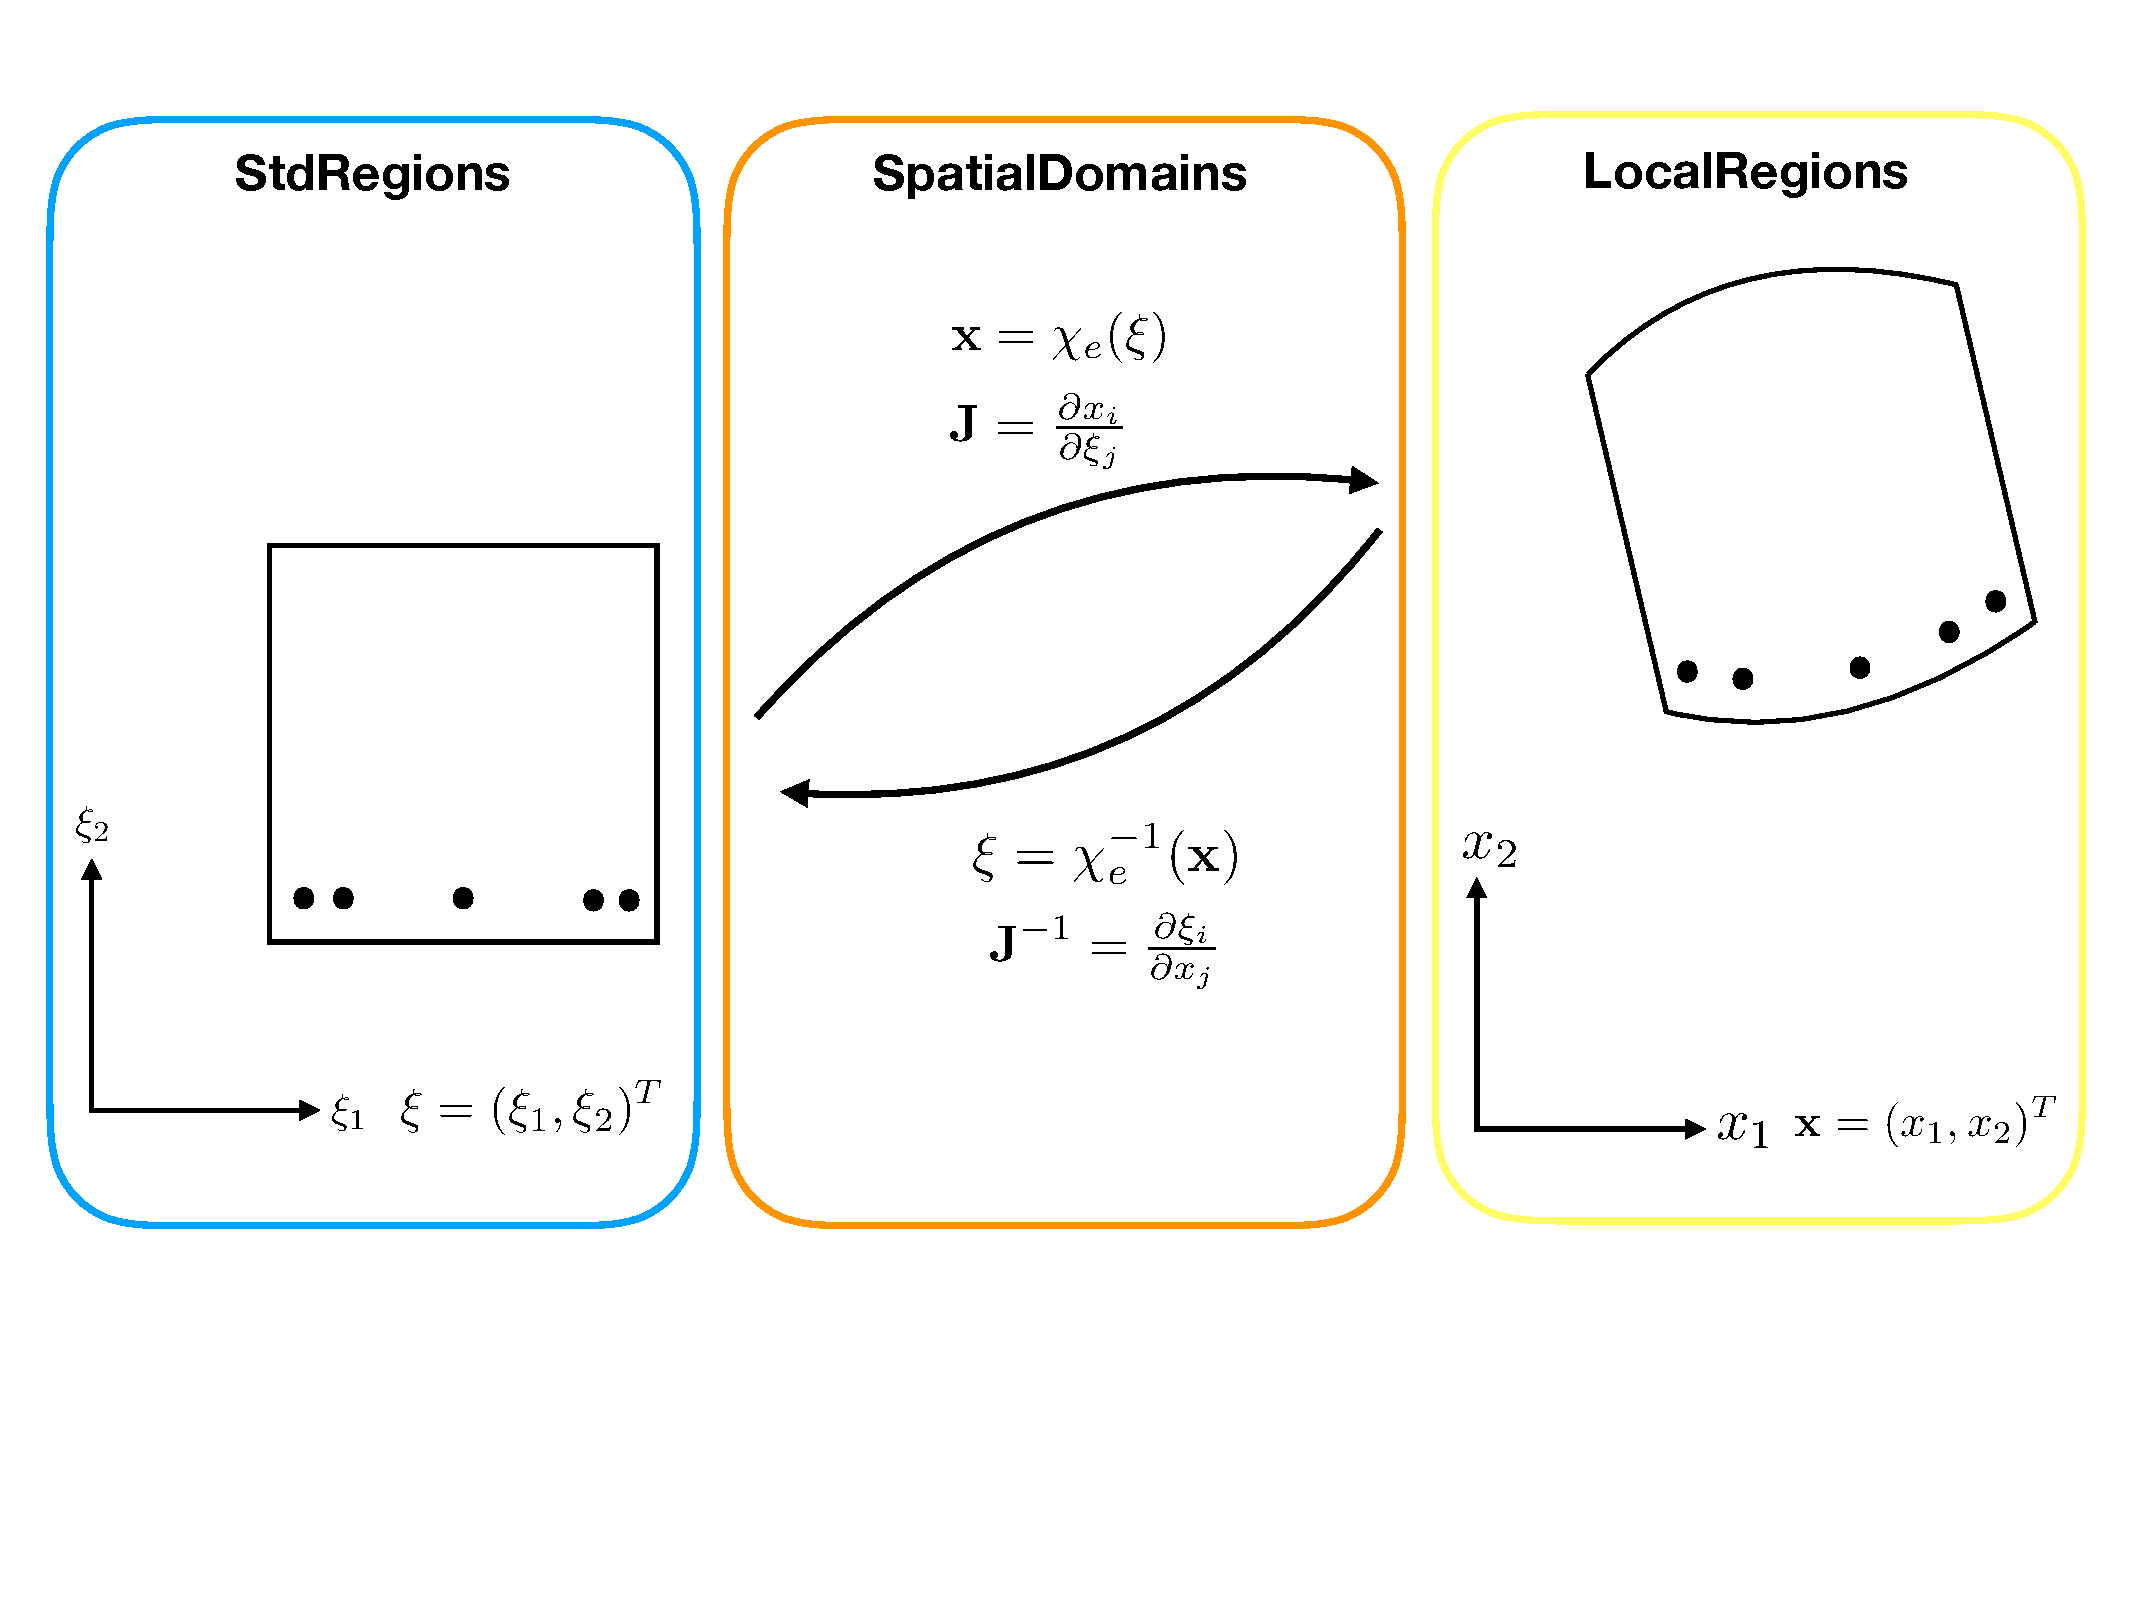
\includegraphics[width=4in]{img/stdtolocal.pdf}
\caption{Diagram showing the LocalRegion (yellow) {\em is-a} StdRegion (blue) which {\em has-a} SpatialDomain (orange) in terms of coordinate systems and mapping functions. This diagram highlights how points (positions in space) are mapped between different (geometric) regions.}
\label{intro:stdtolocal}
\end{figure}

Since $\phi^e(\xi_1,\xi_2)$ lives on ${\mathcal Q} = [-1,1] \times [-1,1]$ (i.e. $\phi^e:{\mathcal Q}\rightarrow\mathbb{R}$) and is for this example polynomial, we can integrate it exactly (to machine precision) using Gaussian integration, and we can differentiate it by writing it in a Lagrange basis and forming a differential operator matrix to act on values of the function evaluated at points.   If the function were not polynomial but instead only a smooth function, we could approximate it with quadrature and decide an appropriate basis by which to 
approximate its derivatives.  All the routines needed for differentiating and integrating polynomials over various standard regions are contained within the StdRegions 
directory (and will be discussed in Chapter \ref{chap:stdregions}).   A local region expansion, such as a basis defined on a quadrilateral element, QuadExp, is a linear combination of basis functions over its corresponding standard region as mapped by
information contained within its spatial domain mapping.  Local region class definitions are in the LocalRegions directory (and will be discussed in Chapter \ref{chap:localregions}).  Using the inheritance language of {\em C++}, we would say that a local region {\em is-a} standard region and
{\em has-a} spatial domain object.  The SpatialDomains directory contains information that expresses the mapping function $\chi_e(\cdot)$ from the standard region
to a local region.  SpatialDomains is explored in Chapter \ref{chap:spatialdomains}.  In the case of our quad example, the SpatialDomain object held by a QuadExp would connect the local region to its StdRegion parent,
and correspondingly would allow integration and differentiation in world space (i.e., the natural coordinates in which the local expansion lives).  If ${\mathcal E}$ denotes our
geometric region in world space and if $F:{\mathcal E}\rightarrow\mathbb{R}$ is built upon polynomials over its standard region, then we obtain $F(x_1,x_2) = \phi^e(\chi_e^{-1}(x_1,x_2))$.  Note that even though $\phi^e$ is polynomial and $\chi_e$ is polynomial, the composition using the inverse of $\chi_e$ is not guaranteed to be polynomial: it is only
guaranteed to be a smooth function. 

Putting this in the context of MultiRegions, we arrive at Figure \ref{intro:structure1}.  The MultiRegions directory (which will be discussed in Chapter \ref{chap:multiregions}) contains various data structures that combine
local regions.  One can think of a multi-region as being a set of local region objects in which some collection of geometric and/or function properties are enforced.
Conceptually, one can have a set of local region objects that have no relationship to each other in space.   This is a set in the mathematical sense, but not really
meaningful to us for solving approximation properties.  Most often we want to think of sets of local regions as being collections of elements that are geometrically
contiguous -- that is, given any two elements in the set, we expect that there exists a path that allows us to trace from one element to the next.   Assuming
a geometrically continuous collection of elements, we can now ask if the functions built over those elements form a piece-wise discontinuous approximation
of a function over our Multiregion or a piece-wise continuous $C^0$ approximation of a function over our Multiregion.

\begin{figure}[htb]
\centering
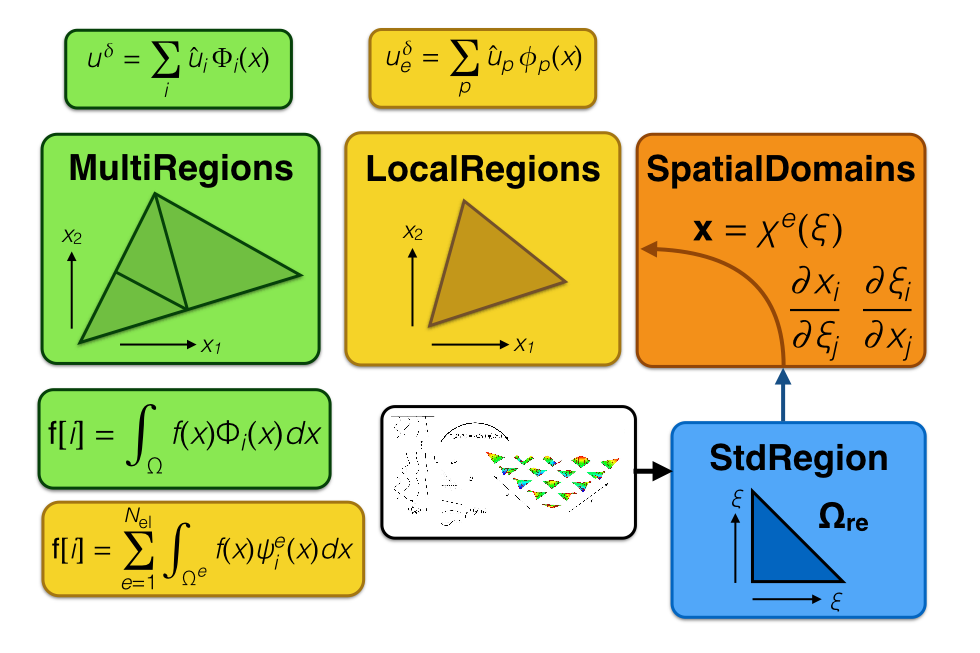
\includegraphics[width=4in]{img/structure1.png}
\caption{Diagram showing how a MultiRegion (green) contains a collection of LocalRegions (yellow), where a LocalRegion {\em is-a} StdRegion (blue) which {\em has-a} SpatialDomain (orange) in terms of coordinate systems and mapping functions.  This diagram highlights the expansions of the solution formed over each geometric domain.}
\label{intro:structure1}
\end{figure}


%%%%%%%%%%%%%%%%%%%%%%%%%%%%%%
\subsubsection{Top-Down Perspective}

The top-down perspective on the library is best understood from Figure \ref{intro:structure2}.  From this perspective, we are interested in understanding 
{\nek} from the solvers various people have contributed.  

\begin{figure}[htb]
\centering
\includegraphics[width=4in]{img/structure2.png}
\caption{Diagram showing the top-down perspective on library components.  Various solvers (along the top) can capitalize on generic SolverUtils and are built upon
the core {\nek} libraries consisting of MultiRegions (green), Collections (red), LocalRegions (yellow), SpatialDomains (orange) and StdRegions (blue).  The most 
generic mathematical and computer science features are contained within LibUtilities, which in part draws from various community resources such as Boost, Metis, etc.}
\label{intro:structure2}
\end{figure}


\section{Assumed Proficiencies}

This developer's guide is designed for the experienced \shp{} user who wishes to go beyond
using various \nek{} solvers and possibly to add new features or capabilities at the library,
solver or utilities levels.  Since the focus of this document is \nek{}, we cannot 
recapitulate all relevant mathematical or computer science concepts upon which our
framework is built.  In this section we provide a listing of areas and/or topics of 
assumed knowledge, and we provide a non-exhaustive list of references to help
the reader see the general areas of additional reading they may need to benefit fully
from this manual.

We assume the reader has a familiarity and comfort-level with the following areas:

\begin{enumerate}
\item Finite Element Methods (FEM) ~\cite{Hughes87,Schwab,BaSzKa81} and more generally the mathematical ideas 
surrounding continuous Galerkin (cG) methods.  This includes basic calculus of variation concepts, basic
partial differential equation knowledge, and general forms of discretization and approximation.

\item Polynomial Methods~\cite{CanutoHQZ87,Funaro92,HGG}, and in particular concepts surrounding polynomial
spaces, basis functions and numerical differentiation and quadrature.

\item Spectral Element Methods (SEM)~\cite{DevilleFM02,KaSh05}.

\item Discontinuous Galerkin Methods \cite{CockburnKS,HesthavenW08}.

\item Scientific Computing~\cite{Heath,KarniadakisK03}.  We assume a graduate-level proficiency in basic
computational techniques such as dealing with numerical precision (accuracy and conditioning), root-finding algorithms,
differentiation and integration, and basic optimization.

\item Linear Algebra \cite{TrefethenB97,Demmel97}.  We assume a strong knowledge of linear algebra and a reasonable 
comfort level with the various numerical algorithms used for the solution of symmetric and non-symmetric linear systems.
\end{enumerate}

\section{Other Software Implementations and Frameworks}

In the last ten years a collection of software frameworks has been put forward to try to bridge the gap between the 
mathematics of high-order methods and their implementation. 
A number of software packages already exist for fluid dynamics which implement
high-order finite element methods, although these packages are typically targeted at a specific
domain or provide limited high-order capabilities as an extension.
A major challenge many practitioners have with
spectral/{\em hp\/} elements and high-order methods, in general, is the complexity (in terms of algorithmic design) they
encounter. In this section, we give an incomplete but
representative summary of several of these attempts to overcome this challenge.

The \emph{Nektar flow solver} is the predecessor to \nek{} and
implements the \shp{} element method for solving the incompressible
and compressible Navier-Stokes equations in both 2D and 3D. While it is widely
used and the implementation is computationally efficient on small parallel problems,
achieving scaling on large HPC clusters is challenging. Semtex \cite{BlSh04}
implements the 2D spectral element method coupled with a Fourier expansion in
the third direction. The implementation is highly efficient, but can only be
parallelised through Fourier-mode decomposition.
Nek5000 \cite{Nek5000} is a 3D spectral element code, based on hexahedral
elements, which has been used for massively parallel simulations up to 300,000
cores. The Non-hydrostatic Unified Model of the Atmosphere (NUMA) \cite{GiraldoKC13} is a spectral element framework that employs continuous 
and discontinuous Galerkin
strategies for solving a particular problem of interest, but in a way on which others could adopt and build.  
Hermes \cite{VeSoZi07} implements hp-FEM for two-dimensional problems and
has been used in a number of application areas. Limited high-order finite
element capabilities are also included in a number of general purpose PDE
frameworks including the DUNE project \cite{DeKlNoOh11} and deal.II
\cite{BaHaKa07}.
% %
FEniCS \cite{FEniCS} is a collaborative project for the development of scientific computing tools, with a particular focus 
on the automated solution of differential equations by finite element methods (FEM).  Through the use of concepts such as meta-programming,
FEniCS tries to keep the solving of PDEs with FEM, from the application programmers' perspective, as close to the mathematical expressions
as possible without sacrificing computational efficiency.
%%
A number of codes also implement high-order finite element methods on
GPGPUs including nudg++, which
implments a nodal discontinuous Galerkin scheme \cite{HeWa07}, and PyFR
\cite{WiFaVi14}, which supports a range of flux reconstruction techniques.

\section{How to Use This Document}

In the next chapter, we will introduce the reader to various computer science tools and ideas upon which we rely heavily in our development and deployment of {\nek}.  The remainder of this developer's guide is then partitioned into three parts.

In Part \ref{part:library}, we provide an overview of the various data structures and algorithms that live within the {\em library} subdirectory.  We think of the library as containing all the basic building blocks of the {\nek} code, as discussed above.  In this part of the developer's guide, we have dedicated a chapter to each subdirectory within the library.  Each chapter contains three main sections.  The first section of a chapter provides an overview of the mathematical concepts and terminology used within the chapter.  This is not meant to be a detailed tutorial, but rather a reminder of basic concepts.  The second section of a chapter provides a detailed description of the data structures introduced in that part of the library.  The third section of a chapter is dedicated to explaining the algorithmic aspects of the library.  Instead of going function by function or method by method, we have decided to structure this section in the style of ``frequently asked questions" (FAQ).  Based upon our long experience with students, postdocs and collaborators, we have distilled down a collection of questions that we will use (from the pedagogical perspective) to allow us to drill down into key algorithmic aspects of the library.

In Part \ref{part:solvers}, we provide an overview of the many solvers implemented on top of the {\nek} library.  Each chapter is dedicated to a different solver, and correspondingly may take on a slightly different style of presentation to match the depth of mathematical, computer science and engineering knowledge to understand the basic data structures and algorithms represented there.

In Part \ref{part:utilities}, we provide an overview of many of the utilities often used in our simulation pipeline -- from things that aid the user in the preprocessing steps such as setting up parameter files and meshing to the postprocessing step of field conversion for visualization.

How you engage with this material is based upon your goals.  If your goal is to:

\begin{itemize}
\item Introduce a new solver, then you would want to jump to Part \ref{part:solvers} and see how other solvers have been built.  Then, depending on what library functions are needed, you may need to step back into the library parts of this manual to understand how to use some of our basic library functionality.
\end{itemize} 







